%% Begin slides template file
\documentclass[11pt,t,usepdftitle=false,aspectratio=169]{beamer}

\usepackage{graphicx}
%% ------------------------------------------------------------------
%% - aspectratio=43: Set paper aspect ratio to 4:3.
%% - aspectratio=169: Set paper aspect ratio to 16:9.
%% ------------------------------------------------------------------

\usetheme[nototalframenumber,foot,logo]{uibk}
%% ------------------------------------------------------------------
%% - foot: Add a footer line for conference name and date.
%% - logo: Add the university logo in the footer (only if 'foot' set).
%% - bigfoot/sasquatch: Larger font size in footer (requires 'foot' to be set).
%% - nofootrule: Removes horizontal ruler above footer line.
%% - nototalframenumber: Hide the total number of frames.
%% - noframenumber: Hide both, frame number and total number of frames.
%% - license: Add CC-BY license symbol to title slide (e.g., for conference uploads)
%%   (TODO: At the moment no other licenses are supported.)
%% - licenseall: Add CC-BY license symbol to all subsequent slides.
%% - url: use \url{} rather than \href{} on the title page
%% - nosectiontitlepage: switches off the behaviour of inserting the
%%   titlepage every time a \section is called. This makes it possible to
%%   use more than one section + thanks page and a ToC off by default.
%%   If the 'nosectiontitlepage' is set you can create UIBK title slides
%%   using the command '\uibktitlepage{}' in your document to create
%%   one or multiple title slides.
%%
%% Default: `[nototalframenumber,foot,logo]`, the footer displays the logo,
%% footer text and date (if set), as well as the frame number.
%% If all options are removed ([]) only the frame number and total frame number
%% are shown. Can be removed as well using [noframenumber].
%% ------------------------------------------------------------------

%% ------------------------------------------------------------------
%% The official corporate colors of the university are predefined and
%% can be used for e.g., highlighting something. Simply use
%% \color{uibkorange} or \begin{color}{uibkorange} ... \end{color}
%% Defined colors are:
%% - uibkblue, uibkbluel, uibkorange, uibkorangel, uibkgray, uibkgraym, uibkgrayl
%% The frametitle color can be easily adjusted e.g., to black with
%% \setbeamercolor{titlelike}{fg=black}
%% ------------------------------------------------------------------

%\setbeamercolor{verbcolor}{fg=uibkorange}
%% ------------------------------------------------------------------
%% Setting a highlight color for verbatim output such as from
%% the commands \pkg, \email, \file, \dataset 
%% ------------------------------------------------------------------


%% information for the title page ('short title' is the pdf-title that is shown in viewer's titlebar)
\title[MyFirstGame]{MyFirstgame}
\subtitle{A fast paced pvp shooter}
%%\URL{www.uibk.ac.at/statistics}

\author[Alan Gallo, Fabian Pfaff]{Alan Gallo, Fabian Pfaff, ex. Balázs Bozsó}
%('short author' is the pdf-metadata Author)
%% If multiple authors are required and the font size is too large you
%% can overrule the font size of author and url by calling:
%\setbeamerfont{author}{size*={10pt}{10pt},series=\mdseries}
%\setbeamerfont{url}{size*={10pt}{10pt},series=\mdseries}
%\URL{}
%\subtitle{}

\footertext{{\LaTeX} beamer theme}
\date{2025-10-14}

\headerimage{6}
%% ------------------------------------------------------------------
%% The theme offers four different header images based on the
%% corporate design of the university of innsbruck. Currently
%% 1, 2, 3, 4, 5, 6 is allowed as input to \headerimage{...}
%% as well as \headerimage{mylogo.png}. Default or fallback is '1'.
%% ------------------------------------------------------------------

\begin{document}

%% ALTERNATIVE TITLEPAGE
%% The next block is how you add a titlepage with the 'nosectiontitlepage' option, which switches off
%% the default behavior of creating a titlepage every time a \section{} is defined.
%% Then you can use \section{} as it's originally intended, including a table of contents.
% \usebackgroundtemplate{\includegraphics[width=\paperwidth,height=\paperheight]{titlebackground.pdf}}
% \begin{frame}[plain]
%     \titlepage
% \end{frame}
% \addtocounter{framenumber}{-1}
% \usebackgroundtemplate{}

%% Table of Contents, if wanted:
%% this requires the 'nosectiontitlepage' option and setting \section{}'s as you want them to appear here.
%% Subsections and subordinates are suppressed in the .sty at the moment, search
%% for \setbeamertemplate{subsection} and replace the empty {} with whatever you want.
%% Although it's probably too much for a presentation, maybe for a lecture.
%% Please note: \maketitle allows you to render a uibk-style title page wherever needed
%% in the document even if 'nosectiontitlepage' option is set (note: \maketitle will not
%% create a new section and is therefore not included in \tableofcontents (if used).
% \maketitle
% \begin{frame}
%     \vspace*{1cm plus 1fil}
%     \tableofcontents
%     \vspace*{0cm plus 1fil}
% \end{frame}


%% this sets the first PDF bookmark and triggers generation of the title page
\section{MyFirstGame}

%% this just generates PDF bookmarks
\subsection{Component Overview}

%% first slide
\begin{frame}
\frametitle{Component Overview}
   
   \bigskip

   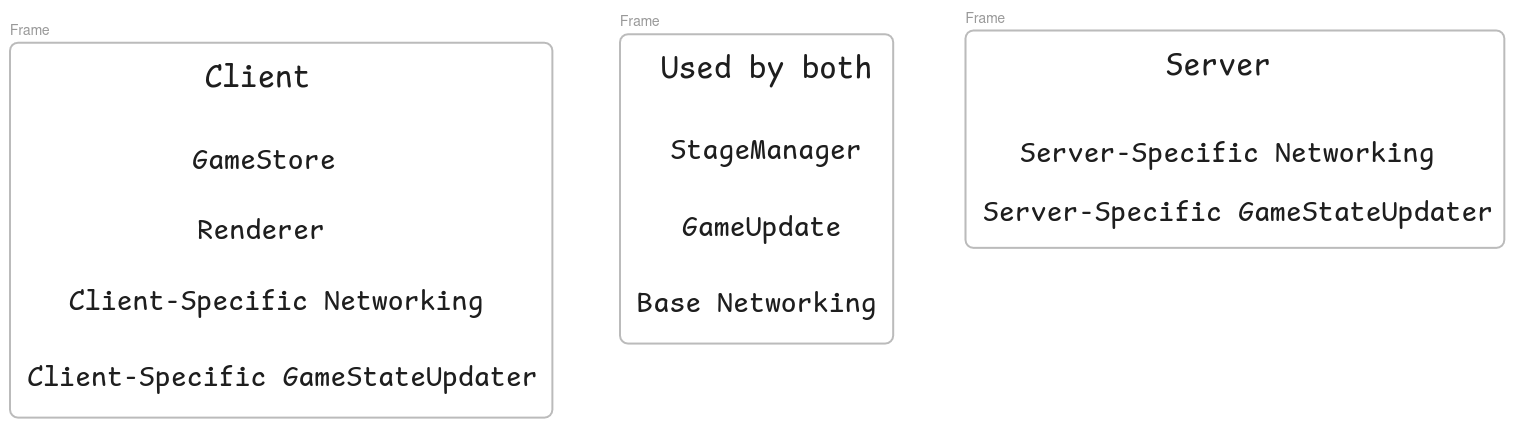
\includegraphics[width=145mm]{customImages/Komponents CPP.png}
\end{frame}

\subsection{Dependencies}

%% first slide
\begin{frame}
\frametitle{Dependencies}

   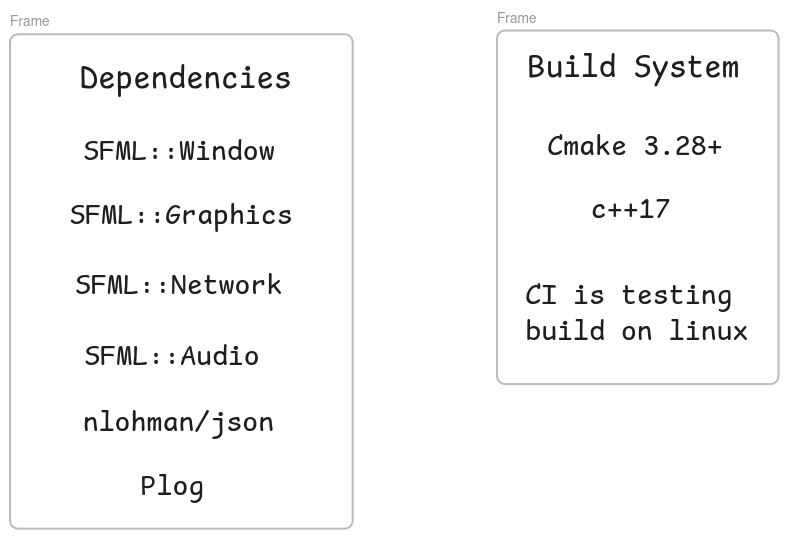
\includegraphics[width=100mm]{customImages/Deps CPP.png}
\end{frame}


\subsection{Code Insight: GameStateStore}
%% first slide
\begin{frame}
\frametitle{Code Insight: GameStateStore}
   \begin{center}
      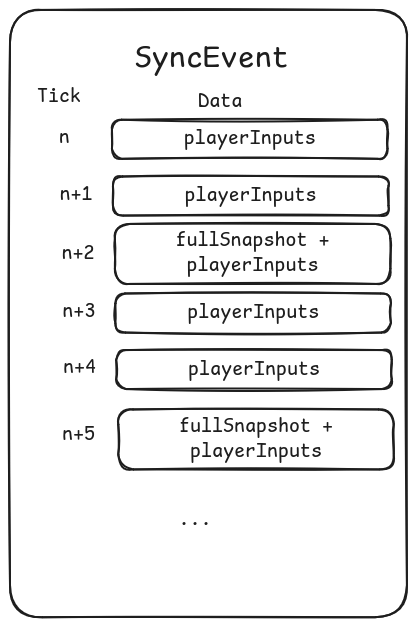
\includegraphics[width=45mm]{customImages/SyncEvent.png}
   \end{center}
\end{frame}
\begin{frame}
\frametitle{Code Insight: GameStateStore}
   \bigskip
   
   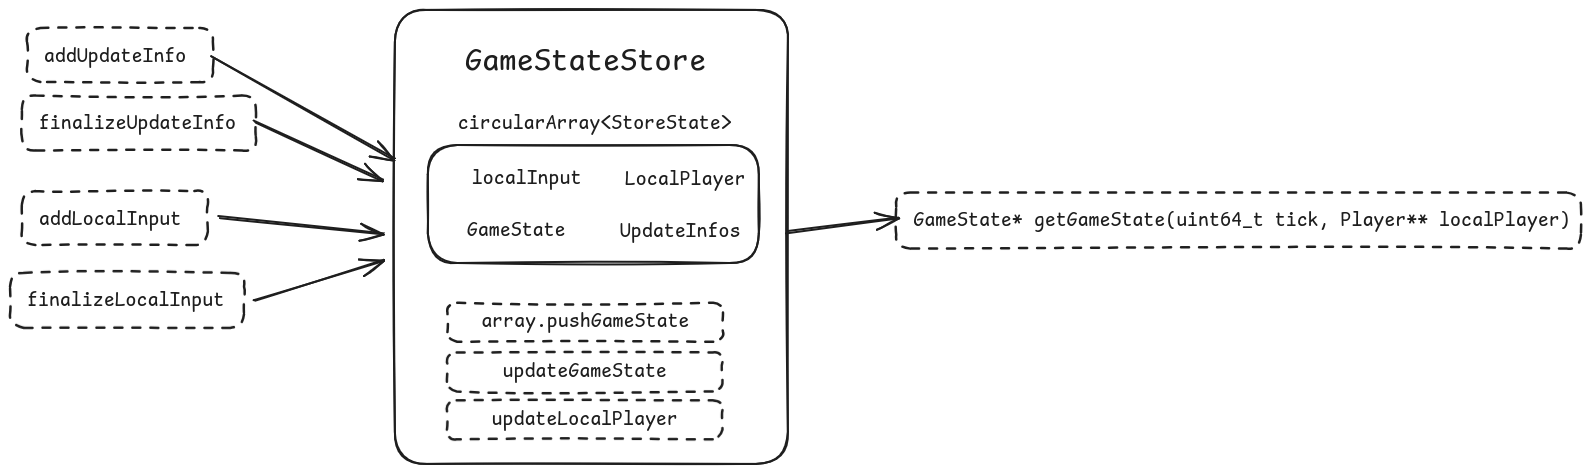
\includegraphics[width=145mm]{customImages/GameStore.png}
\end{frame}


\subsection{Code Insight: GameUpdates}
%% first slide
\begin{frame}
\frametitle{Code Insight: GameUpdates}
   \begin{center}
      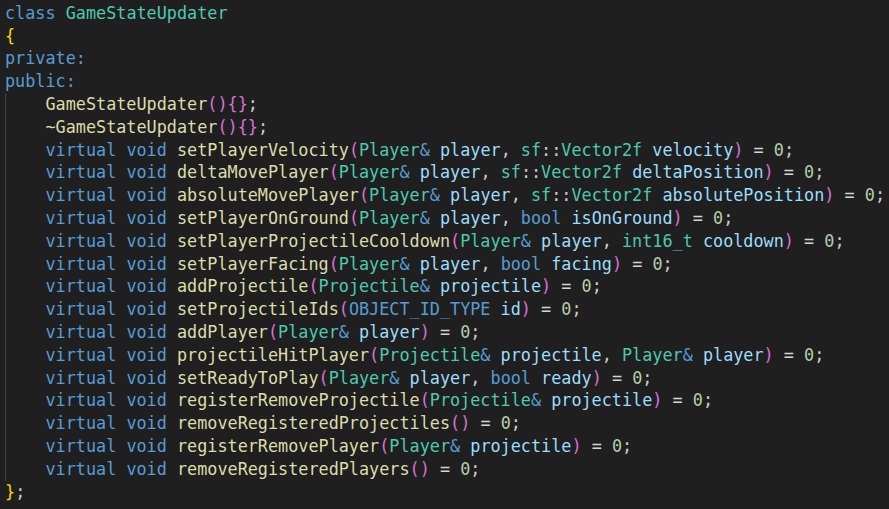
\includegraphics[width=100mm]{customImages/Screenshot_Interface.png}
   \end{center}
\end{frame}

\begin{frame}
\frametitle{Code Insight: GameUpdates}
\bigskip
\bigskip
   \begin{center}
      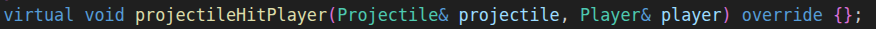
\includegraphics[width=85mm]{customImages/Screenshot_Client.png}
      \bigskip
      
      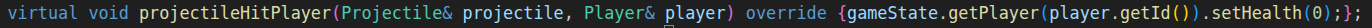
\includegraphics[width=145mm]{customImages/Screenshot_Server.png}
   \end{center}
\end{frame}

%% next PDF bookmark
\subsection{Lessons learned}

\begin{frame}[fragile]
\frametitle{Lessons learned}

   \textbf{Planning before implementing}
   \bigskip
   
   \textbf{First Multiplayer is hard}
   \bigskip

   \textbf{Debugging is useful}
\end{frame}


\subsection{Live Demo}

\begin{frame}[fragile]
\frametitle{Live Demo}
\end{frame}


%% to show a last slide similar to the title slide: information for the last page
\title{Thank you for your attention!}
\subtitle{}
\section{Thanks}

\end{document}

